\documentclass[a4paper,11pt,titlepage]{article}
\usepackage{amssymb}
\usepackage{hyperref}
\usepackage{booktabs}
\usepackage{geometry}
\usepackage{listings}
\usepackage{graphicx}
\usepackage{natbib}
\usepackage{todonotes}
\usepackage{enumitem}
\usepackage{multirow}
\usepackage{tikz}
\usepackage{fancyhdr}
\usetikzlibrary{arrows,decorations.pathmorphing,backgrounds,positioning,fit,petri,matrix,folding}

\setlength\headheight{20pt}
\addtolength\topmargin{-10pt}
\addtolength\footskip{20pt}

\fancypagestyle{plain}{%
\fancyhf{}
\fancyfoot[RO,LE]{\sffamily\bfseries\thepage}
\renewcommand{\headrulewidth}{0pt}
\renewcommand{\footrulewidth}{1pt}
}


\newcommand{\HRule}{\rule{\linewidth}{0.5mm}}

\newcommand{\uni}{Eindhoven University of Technology}
\newcommand{\fase}{Computer Science and Engineering}
\newcommand{\vak}{Business Process Simulations}
\newcommand{\vakcode}{2II75}
\newcommand{\essaytitle}{Large Fuel Station Analysis}
\newcommand{\stad}{Eindhoven}
\newcommand{\tbsep}{\ \ \textbar \ \textbar \ \textbar \ \textbar \ \textbar \ \textbar \ \textbar \ \textbar \ \textbar \ \textbar \ \ }

\pagestyle{fancy}
\fancyhf{}
\fancyhead[RO,LE]{\vak}
\fancyhead[LO,RE]{\uni}
\fancyfoot[RO,LE]{\sffamily\bfseries\thepage}
\fancyfoot[LO,RE]{\essaytitle}
\renewcommand{\headrulewidth}{1pt}
\renewcommand{\footrulewidth}{1pt}

\bibliographystyle{plain}
\hypersetup{pdfborder={0 0 0}}

\setlength{\parskip}{10pt}

\geometry{
	includeheadfoot,
	margin=2.54cm
}
\author{
	Nicky Advokaat (0740567) - \texttt{n.advokaat@student.tue.nl}
	\and
	Robbert Jongeling (0747896) - \texttt{r.m.jongeling@student.tue.nl}
	\and
	Bram Kohl (0746107) - \texttt{b.j.e.kohl@student.tue.nl}
	\and
	Jasper Selman (0741516) - \texttt{j.w.m.selman@student.tue.nl}
	\and
	Ramon de Vaan (0758873) - \texttt{r.d.vaan@student.tue.nl}
}
\date{\today}

\begin{document}
	\begin{titlepage}
	\begin{center}

% Upper part of the page
		\includegraphics[width=0.15\textwidth]{images/tuelogo}\\[1cm]

		\textsc{\LARGE \uni}\\[0.2cm]

		\textsc{\fase}\\[1.6cm]

        \textsc{\LARGE \vak}\\[0.5cm]

% Title
\HRule \\[0.4cm]
{ \huge \bfseries \essaytitle}\\[0.4cm]

\HRule \\[1.5cm]

% Author and supervisor
	\emph{Group 13:}\\
    \begin{tabular}{l l l}
	Nicky \textsc{Advokaat} & 0740567 & \href{mailto:n.advokaat@student.tue.nl}{\texttt{n.advokaat@student.tue.nl}}\\
	Robbert \textsc{Jongeling} & 0747896 & \href{mailto:r.m.jongeling@student.tue.nl}{\texttt{r.m.jongeling@student.tue.nl}}\\
	Bram \textsc{Kohl} & 0746107 & \href{mailto:b.j.e.kohl@student.tue.nl}{\texttt{b.j.e.kohl@student.tue.nl}}\\
	Jasper \textsc{Selman} & 0741516 & \href{mailto:j.w.m.selman@student.tue.nl}{\texttt{j.w.m.selman@student.tue.nl}}\\
	Ramon \textsc{de Vaan} & 0758873 & \href{mailto:r.d.vaan@student.tue.nl}{\texttt{r.d.vaan@student.tue.nl}}
    \end{tabular}
		\vfill

% Bottom of the page
		{\large \today} \\
		\stad

	\end{center}
\end{titlepage}
    \tableofcontents
    \listoftables
    \listoffigures
    \newpage
	\section{Executive Summary}
Bill Perterson of BP fuel wants to open a new large fuel station. In this fuel station there are lanes before the pumps in which vehicles queue up, and cash registers after the pumps to pay for the gas.  Bill has assigned us the task of creating a cashier schedule for the registers. He wants to minimize his expenses in paychecks, but the schedule also has to meet the following requirements:

\begin{enumerate}
\item Cars (with  trailers) typically spend at most 30 minutes from arrival to departure.
\item Trucks typically spend at most 45 minutes from arrival to departure.
\item At most 1$\%$ of the arriving vehicles will be blocked. A vehicle is blocked when the lanes before the fuel pumps are full.
\end{enumerate}

\noindent The trivial solution of always keeping all checkouts open meets all of these requirements. 
No cars will be blocked and the throughput time of the cars and trucks will be low.
However, if all the checkouts will be occupied, the costs in paychecks will be around \EUR{3200} per day, which is unacceptable.
Instead, an optimal solution has to be found such that the schedule meets the requirements stated above, while the cost of the cashiers scheduled is minimized.

\noindent Using simulation techniques various feasible solutions were found. The best solution is described in detail in section 9. 
This solution has a total cost of \EUR{2242,50} per day, which is about \EUR{900} less than the trivial solution. 
Since a cashier costs about \EUR{100} a day, we have almost cut away one third of the total amount of cashiers. 
In this case both the cars and trucks spend on average less than half an hour in the fuel station and only 0.53\% of all vehicles get blocked.

\noindent A decreasing demand of fuel in the future caused by more fuel efficient cars can cause a drop of 20\% both in the demand for fuel as well as in the arrival rate of cars. Simulating this new situation gives us a schedule that has a total cost of \EUR{1767,50}. This is a drop of 20\% compared to the original costs. This seems good, but the total profit has decreased a little more than 20\%, because both the fuel amount and the arrival rate dropped with 20\%.
    \newpage
	\section{Introduction}
Despite the rapid depletion of fossil fuel resources, and the rise of the electric vehicle industry, the fuel station industry remains big business.
As a result, Bill Peterson of BP fuel is opening a new, very large fuel station in Luxemburg.
Bill has a specific layout in mind: the fuel station will have 15 fuel pumps divided in 5 groups of 3 pumps each, where every group will have a single cashier.
Vehicles will queue in one of the 15 lanes and wait for their turn at the pump.
Afterwards, they will head to the associated cashier to pay.

Since Bill lacks experience in scheduling the workers in the specified fuel station layout, we, group 13, have been hired as a consultant to tackle that problem.
Obviously, our goal is to maximize the profit of the fuel station, whilst satisfying several requirements made by Bill regarding customer satisfaction.
We are, however, limited in certain aspects.
First of all, fuel prices are fixed in Luxemburg, so we cannot reduce or increase prices to either get more customers or increase profit per customer.
As a result, the only way for us to increase the profit, is to reduce the cost of the fuel station, by changing the schedule of the workers.
Luckily, Bill has collected many statistics about vehicles entering one of his competitor's fuel stations and has recorded information about fuel amounts in some of his other fuel stations.

In this report we will analyse the problem described above, to provide a base on which we will later deliver a recommendation regarding not only the current situation, but possible future situations, if his needs were to change.
We will attempt to do so, firstly by describing the system in detail, making assumptions on things that were not explained fully.
Next, we will analyse the input provided to us, trying to fit statistical models to the data.
Finally, we will provide conceptual models by all group members individually.
	
	\section{System Description}
In this section we give a description of the fuel station.
First, we describe all key object classes appearing in the model and their associated actions. 
Next, performance indicators are listed.
Thirdly, we pose questions to be answered by our research.
Finally, we name alternative solutions to achieve Bills goals.

\subsection{Key Object Classes}
In our fuel station we can distinguish several key object classes.
Table \ref{tab:koc} shows all key object classes as well as their types and states.
The classes we distinguish are \textit{Vehicle}, \textit{Lane}, \textit{Employee}, \textit{Pump} and \textit{Queue Spot}. 

The class \textit{Vehicle} consists of three types: \textit{Car, Car with Trailer} and \textit{Truck}.
 Vehicles are in one of six states while they are in the fuel station. 
 The first state is \textit{Arriving}, a vehicle in this state has entered the fuel station but has not yet chosen any queue to enter.
 A vehicle in the next state, \textit{In Queue}, has chosen a queue and is waiting in line. 
 The third state, \textit{Refueling}, indicates that the vehicle has reached the pump and is now refueling. 
 The fourth state, \textit{Waiting for Cashier} means the vehicle is done refueling, but has not reached the cashier yet. 
 The next state, \textit{Paying}, means the vehicle has reached the cashier and payment is being handled. 
 When a vehicle is in the last state, \textit{Idle}, it has outside our station i.e. it has not yet arrived or has already left.
 
The second class is \textit{Lane}, it consists of a single type, also named \textit{Lane}.
A \textit{Lane} is a queue in front of the pumps and is in one of two states. 
The first state is \textit{Available}, i.e. vehicles can enter the lane.
The second state is \textit{Closed}, i.e. no vehicle can enter the lane.
We assume that within groups of three lanes, the state is shared, i.e., in every group either all lanes are opened or all lanes are closed.

The third class is the \textit{Employees}, in this model we consider only one type of employee, \textit{Cashier}. 
A cashier can be in one of four states.
The first state is \textit{Off-duty}, i.e. the cashier is not working at the moment. 
Secondly, there is the state \textit{Available}, the cashier is on duty but he is not serving customers at the moment. 
When he is busy serving a customer he is in the third state, \textit{Serving}.
The last state a cashier can be in is the state \textit{Restocking Supplies}. 
This means the shift of the cashier has ended but he is restocking the supplies.

The fourth class is \textit{Pump}.
Each of these pumps can be either in the \textit{Available} or \textit{In Use} state.
We assume that each pump is capable of providing fuel at low and high speed, depending on the vehicle type.
Furthermore we assume that there is enough fuel stored to ensure a continuous flow.

The last class is \textit{Queue Spot}. 
This class represents the spots which are available between the pumps and the cashier. 
There are three kinds of spots. 
\textit{First Spot} is the spot right after the pump and there are three of them for every group of three lanes a served by a single cashier.
\textit{Second  Spot} is the spot after \textit{First Spot} and there are only two of them for every group of three lanes. 
\textit{Third Spot} is the last spot and also the spot where a vehicle is served by a cashier, there is only one of them for every group of three lanes. 
Every one of these spots can either be occupied by a vehicle or be free, hence the states \textit{Occupied} and \textit{Free}.

\begin{center}
\begin{table}[h]
\begin{tabular}{| l | l | l | l | l |}
\hline
\textbf{Vehicle} & \textbf{Lane} & \textbf{Employee} & \textbf{Pump} & \textbf{Queue Spot}\\
\hline
\textbf{Types} & \textbf{Types} & \textbf{Types} & \textbf{Types} & \textbf{Types}\\
- Car & - Lane & - Cashier& & - First Spot\\
- Car with Trailer & & & & - Second Spot\\
- Truck & & & & - Third Spot\\
& & & & \\
\textbf{States} & \textbf{States} & \textbf{States} & \textbf{States} & \textbf{States}\\
- Arriving & - Available & - Off-duty & - Available & - Free\\
- In Queue & - Closed & - Available & - In Use & - Occupied\\
- Refueling & & - Serving & &\\
- Waiting for Cashier & & - Restocking Supplies & &\\
- Paying & & & &\\
- Idle & & & &\\
\hline
\end{tabular}
\caption{Key Object Classes}
\label{tab:koc}
\end{table}
\end{center}

\subsection{Actions}
We model six actions that occur in the system.
Each of these actions causes a number of state changes, depending on the state the system is in when the action occurs. 
Below we enumerate these actions along with the state changes they cause.

\begin{enumerate}
	\item \textbf{A vehicle arrives}
	\begin{enumerate}
		\item Vehicle state changes from \textit{Idle} to \textit{Arriving}.
		\item If every lane is either \textit{Closed} or there is insufficient space for the arriving vehicle, then the vehicle becomes \textit{Idle} again.
		\item If a lane is \textit{Available} and the Pump is \textit{Available} (No Vehicle using or blocking it) then:
	\begin{enumerate}
		\item The Pump goes from \textit{Available} to \textit{In Use}.
		\item The Vehicle goes from \textit{Arriving} to \textit{Refueling}
	\end{enumerate}
	Assumption: If a Pump is \textit{Available}, the Lane is empty (i.e. when a Vehicle stops blocking it, the next Vehicle starts using it at the same time).
	\item If a lane is \textit{Available} and there is enough space for the arriving Vehicle and the Pump is \textit{In Use} then the Vehicle goes from \textit{Arriving} to \textit{In Queue}
	\end{enumerate}
	
	\item \textbf{A cashier starts a shift}
	\begin{enumerate}
		\item If there is no Vehicle at the Third Queue Spot of the Cashier, the Employee goes from \textit{Off-duty} to \textit{Available}.
		\item If there is a Vehicle at the Third Queue Spot of the Cashier, the Employee goes from \textit{Off-duty} to \textit{Serving}.
		\item If the Lanes the cashier is working on are \textit{Closed}, they change to \textit{Available}.
	\end{enumerate}
	
	\item \textbf{A cashier's regular shift ends}
	\begin{enumerate}
		\item If another cashier takes over, the Employee whose shift ends goes from \textit{Available} or \textit{Serving} to \textit{Restocking Supplies}
		\item If no cashier takes over then
		\begin{enumerate}
			\item The Lanes of the cashier go from \textit{Available} to \textit{Closed}
			\item If the Lane and the Queue Spots are empty, the Employee goes from \textit{Available} to \textit{Restocking Supplies}
		\end{enumerate}
	\end{enumerate}
	
	\item \textbf{A cashier finishes Restocking Supplies}
	\begin{enumerate}
		\item{The Employee goes from \textit{Restocking Supplies} to \textit{Off-duty}}
	\end{enumerate}
	
	\item \textbf{A vehicle finishes refueling}
	\begin{enumerate}
		\item If there are \textit{Free} Queue Spots the Vehicle can move to, the Queue Spots go from \textit{Free} to \textit{Occupied}
		\item If the Vehicle can move completely to the Queue Spots of the cashier, and there is a Vehicle waiting in the Lane then the waiting Vehicle goes from \textit{In Queue} to \textit{Refueling}
		\item If the Vehicle can move completely to the Queue Spots of the cashier and there is no Vehicle waiting in the Lane, the Pump goes from \textit{In Use} to \textit{Available}.
		\item If the cashier of the Lane the Vehicle is in is \textit{Available} then:
		\begin{enumerate}
			\item The Vehicle goes from \textit{Refueling} to \textit{Paying}
			\item The Employee of the Lane the Vehicle is in goes from \textit{Available} to \textit{Serving}
		\end{enumerate}
		Assumption: If the cashier is \textit{Available}, there are no Vehicles in his Queue Spots (i.e. when an Employee would become \textit{Available} with Vehicles in his Queue Spots, he becomes/stays \textit{Serving} instead).
		\item If the cashier of the Lane the Vehicle is in is \textit{Serving}, then the Vehicle goes from \textit{Refueling} to \textit{Waiting for Cashier}.
		%If lane can be blocked, check if it can be unblocked here
	\end{enumerate}
	
	\item \textbf{A vehicle has payed}
	\begin{enumerate}
		\item The Vehicle goes from \textit{Paying} to \textit{Idle}.
		\item If there are Vehicles in the Queue Spots of the cashier then:
		\begin{enumerate}
			\item One of those Vehicles changes from \textit{Waiting for Cashier} to \textit{Paying}
			\item If a Vehicle can move further in the Queue Spots causing a Pump to no longer be blocked, then that Pump goes from \textit{In Use} to \textit{Available}
			\item If Queue Spots open up due to Vehicles moving, they go from \textit{Occupied} to \textit{Free}
		\end{enumerate}
		\item If there are no Vehicles in the Queue Spots of the cashier, then the Employee goes from \textit{Serving} to \textit{Available}
		\item If the Lanes of the cashier are \textit{Closed} and the \textit{Queue Spots} of the cashier are all \textit{Free}, and if less than 10 minutes passed since the cashier's regular shift ended the Employee goes from \textit{Serving} to \textit{Restocking Supplies}. 
		\item If the Lanes of the cashier are \textit{Closed} and the \textit{Queue Spots} of the cashier are all \textit{Free}, and if at least 10 minutes passed since the cashier's regular shift ended, the Employee goes from \textit{Serving} to \textit{Off-duty}. 
	\end{enumerate}
\end{enumerate}

\subsection{Performance Indicators:}
The performance indicators which are of use to us are the following:
\begin{itemize}[noitemsep, topsep=0pt]	
\item Average throughput times
\item Average resource utilization
\item Minimum / average / maximum queue sizes
\item Cashier costs
\item Average waiting time before pump
\item Average waiting time after pump
\end{itemize}
The average throughput time is necessary to measure how long cars and trucks need to wait for the pump on average before they are done. 
The customer has a demand that a car or a truck does not have to wait any longer than a given amount of time. 
We use the average throughput time to measure if our model complies with this demand. 

The average resource utilization tells us how well we are using the available resources. 
If the average resource utilization is very low, we have too many cashiers on duty.
We would like it if this number is very high.
The size of the queues tell us if we are using enough or to much resources. 
If the sizes are very large it might be a good idea to put an extra cashier on duty, and if the sizes of the queues are small we might put one cashier less on duty. 
It might also be a convenient to know the minimum and maximum sizes of the queues.

The cost of the cashiers are very important, since they determine how high the expenses are and therefore determine how much of the profit will disappear. 
The last two indicators which might be interesting are the average waiting time before and after the pump. 
These times can show us where the bottlenecks of the fuel station are located. 

\subsection{Questions to be answered}
There are two questions that our simulation study needs to answer. 
The most important question is: "\textit{What is the most cost effective cashier schedule that satisfies the customer requirements?}". 
The second question is \textit{How should the cashier schedule be adopted to the expected decreases in customer demand?}", since vehicles are becoming more and more fuel-efficient.

These questions can be divided in sub-questions, "\textit{What should be the expected waiting times for trucks and cars?}" and "\textit{What is the percentage of blocked vehicles entering the fuel station?}". 
Another question is \textit{"What is the required number of cashiers per shift?}"
These are all questions which can be used to answer the first question. 
To answer the second question we can in fact use the same sub-questions, we only need different data, since the number of arrivals are very different. 

\subsection{Solution Alternatives}

	
	\section{Input Analysis}

In this section we analyze the data that has been collected. One data set contains arrival times of vehicles from the last month. An other file has numbers of the amount of fuel a was needed by a vehicle.  Figures and tables are included in Appendix \ref{app:inputanalysis}.

\subsection{Arrival Times}

We have a raw data set containing arrival times of vehicles at the station over a course of 30 days. 
A histogram of the number of arrivals over time is shown in Figure \ref{fig:histogram-arrivals}. 
Fitting analysis has shown that a Beta distribution is the best fit for this data, a summary of the Fit all functionality of Arena Input Analyzer is shown in Table \ref{tab:fitallarrivals}. 
Fitting a single distribution might not be very useful though. 
We can see that the busiest periods are around 7 AM and 6 PM. 
So it would be more interesting to fit distributions around these times. 

\subsection{Fuel Amounts}

In the fuel amounts dataset, we see a clear difference between cars and trucks.
We consider the fuel needed by cars and by trucks separately, in order to get a better fit of the data.
A histogram of all fuel amounts is shown in Figure \ref{fig:histogram-amounts-unfiltered}, here the high peak corresponds to fuel needed by cars, the lower bars correspond to fuel needed by trucks.
In Figure \ref{fig:histogram-amounts-filtered}, a histogram is shown of only the car data, here the maximum data value has been set to 100.
Figure \ref{fig:histogram-amounts-filtered-trucks} shows the fuel amounts needed by trucks, here the minimum data value has been set to 100.
In Table \ref{tab:fitallamounts} summaries of \textit{Fit all} of the Arena Input Analyzer are shown.
The car data in itself is best described by a normal distribution, all data is best described by a Lognormal distribution, where all car data is compressed into one bar of the histogram.






	
    \section{Simulation Model Description}

In this section the Arena model is described and explained. The model has been split into two models, firstly the management of the cashiers (main model) and secondly the management of the vehicles (submodel Pumps). The used variables, attributes and schedules will be described as well.

\subsection{Cashier management}
A screenshot of the complete cashier management model can be found in figure \ref{fig:model-cashier} in appendix \ref{app:modeldescription}.

This part of the model handles the checkouts and cashiers who work at them. It creates checkouts and assigns numbers to those (between 1 and 5, for the five checkout counters). A checkout is released just before a shift ends, so that it becomes available for an employee starting the shift after the current cashier, and so the new cashier can take over this checkout. When a checkout is released, an OnChange is triggered which puts it in the queue for seizing a cashier again. The creation of checkouts and assigning numbers can be seen in figure \ref{fig:createcheckouts}

\begin{figure}[h!]
	\includegraphics[scale=1]{images/model-description/checkout-creation.PNG}
	\caption{Modeling of the creation of checkouts.}
	\label{fig:createcheckouts}
\end{figure}

Then those checkouts seize a cashier (if available). If there are more than 5 cashiers active at the time, which can happen due to the checkout being released just before a shift ends and being seized by another cashier, the checkout is held at another queue called "Active Cashiers smaller than 5?". If this is not the case the checkout opens the lanes belonging to it. This part of the model can be seen in figure \ref{fig:seizeandopen}

\begin{figure}[h!]
	\includegraphics[scale=1]{images/model-description/seize-and-open.PNG}
	\caption{Modeling of the cashier seizing and checkout opening.}
	\label{fig:seizeandopen}
\end{figure}

After that the checkout has to wait for the cashier to finish his/her shift. This process can be seen in figure \ref{fig:workshift}. In the process, we first check whether it's a 2 hour or a 4 hour shift. The 2 hour shift only occurs when a cashier starts working at 10 p.m. and thus finishes his shift at 2 a.m. the next day. So he actually works a 4 hour shift, but for the current day, he only works from midnight until 2 a.m.
Apart from this exception, the delay is also 5 minutes short of these 2 or 4 hours. After this too short delay, the checkout is released ("Trigger OnChange") and the remaining 5 minutes delay are invoked.
When the cashier is completely done with his regular shift we decrease the number of active cashiers so the possibly stuck checkout can be let through the "Active Cashiers smaller than 5?" state we saw before.

\begin{figure}[]
	\includegraphics[scale=1]{images/model-description/work-shift.PNG}
	\caption{Modeling of the delay for the cashier working his/her shift.}
	\label{fig:workshift}
\end{figure}

After the regular shift, we have to determine what will happen to the lane and cashier. Does he close the lanes and continue working at the checkout? Or does another cashier take over and can he go over to restocking the supplies? This is checked in the blocks displayed in figure \ref{fig:determinetakeover}. As you can see, the check whether someone takes over is split into two checks. This is due to a technicality issue: when checking whether there is a new cashier that takes over the checkout, we check whether the checkout is taken again after the current cashier seized it (which can happen due to releasing the checkout 5 minutes before the end of the shift). This would mean the checkout would be taken over. In order to check this, we store the time each checkout is last seized (this is done in the "open checkout" block in figure \ref{fig:seizeandopen}) and then see if this was later than 3.5 hours ago. But this would not work if we were just starting out the day, e.g. between shift 12 and 1 and shift 1 and 2. Therefor we added another decide block which checks the time.
Then, the pump stays open module can check whether the checkout has been seized again and based on that decide what happens: the lane closes and the cashier stays, or the lane stays open and the cashier can start restocking.

\begin{figure}[]
	\includegraphics[scale=1]{images/model-description/determine-takeover.PNG}
	\caption{Modeling of the check whether a checkout is taken over.}
	\label{fig:determinetakeover}
\end{figure}

The last part of the cashier management is rather straightforward (figure \ref{closerestockandrelease}): based on the previous decision, the checkout is closed after which the cashier works until the lane and checkout queue are both empty after which he restocks the supplies if less than 10 minutes have passed since the checkout closing (which is calculated by setting a variable to the current time upon closing and comparing it to current time after the queue is emptied). Or the checkout does not close and the cashier immediately restocks the supplies.
After this the cashier is released and the checkout entity disposed of.

\begin{figure}[]
	\includegraphics[scale=1]{images/model-description/close-restock-release.PNG}
	\caption{Modeling of the check whether a checkout is taken over.}
	\label{fig:closerestockandrelease}
\end{figure}



	\section{Verification and Validation}

In this Section, the model is verified and validated.
In the verification, the correctness of the model is analysed, in the validation, the model is compared to the assignment description.
More verification and validation can be done when the model reports more statistics.

\subsection{Verification}
Sanity checks, an evaluation of Little's formula and an evaluation of the PASTA property have been done in order to verify the correctness of the model. 
All checks have been done by running the model once with a length of 30 days. 

\subsubsection{Sanity checks}

The total number of arrived vehicles is 61270.
This is the sum of the number of arrived cars (42961), the number of arrived cars with trailers (9049) and the number of arrived trucks (9260).
It is also verified that vehicles choose the shortest queue on arrival by looking at animation while running the simulation.

\subsubsection{Little's formula}
Little's formula states that the average number of jobs in the system, $N$, is equal to the product of the arrival rate $\lambda$ and the average time a job spends in the system, $W$.

For the whole system, we get that the average number of cars arriving per day is 61270/30 = 2042.33. 
If we divide this by the number of opening hours per day (24), we get an arrival rate of 2042.33/24 = 85.0972 vehicles per hour.
The average total time a vehicle is in the system is reported to be 1.2801 hours.
The average number of vehicles in the system (WIP) is reported to be 108.92.
We can see that Little's law holds as:
$$N=\lambda W = 108.933 = 85.0972\cdot1.28010 \approx 108.920.$$

\subsubsection{PASTA property}
The PASTA (\textit{Poisson Arrivals See Time Averages}) property holds when the arrival stream is a Poisson process.
From the Arena help, we know that ``If \textit{Schedule} type is Arrival, the SCHEDULES element defines a time-dependent schedule of entity arrival rates. (\ldots)
An exponential distribution is used to evenly distribute the \textit{Value} arrivals over each hour."
So the time between events has an exponential distribution.
Poisson processes are processes in which events occur at an average rate (the schedule value) but between the events, the time has an exponential distribution.
We conclude that the arrival of vehicles in our model is a Poisson process and thus that the property holds.

\subsection{Validation}
Here, the results of a simulation are compared to the values as provided in the assignment description.
We run the model in the situation where all lanes are always open, again the simulation was run once, with a length of 30 days.

Of the total of arrived vehicles (61720), 42961 where cars. 
This corresponds to 70.1\%, as expected.
Also the number of cars with trailers (9049, 14.8\%) and the number of trucks (9260, 15.1\%) correspond to the expected numbers.


	\section{Experiment Setup}
As stated before, we are trying to increase profit in the fuel station model.
However, we are limited in ways to do so: we cannot alter the fuel cost, nor is there any way for us to increase customer count.
The only way for us to increase profit, is to lower the cost of fuel station operation, by changing the schedule of the workers. \\
Obviously, it would be cheapest not to have workers at all, but we are to adhere to certain requirements regarding customer satisfaction statistics.
For example, the amount of vehicles that are blocked, by all active lanes being full, may not exceed $1\%$ of all arrived vehicles. \\
This gives rise to some conflicting methods of scheduling.
On the one hand, we can increase income by keeping the blocked percentage as low as possible, conversely, the extra cashiers needed would increase cost as well.
Since we were not given the price of fuel, or any of other services offered, for that matter, we cannot calculate the profit increase.
However, we were given the cost of workers for the fuel station. \\
As a result, we will focus entirely on reducing cost by adjusting the worker schedule as much as possible, even though this might not necessarily yield the optimized profit, depending on fuel and service prices.
As such, in our case, finding the optimal solution to the model means finding the minimal cost schedule, whilst still adhering to the requirements that were imposed.
In this section, we will discuss how we intend to find the optimal solution to our model. \\

In our experiment, we will be using the OptQuest tool that Arena offers natively to find an optimal solution.
Our model contains several decision variables, that we can alter to find the optimal solution.
However, doing so by hand would be very labour intensive indeed.
Moreover, there are constraints that limit our solution space, having to check those would require even more of an effort.
Instead, OptQuest allows us to set bounds to decision variables, and constraints, iterating smartly over the large solution space to maximize an objective variable. \\

As described above, the only decision variables we have are the schedules of the cashiers.
We have 12 shift resources, which define the number of cashiers in each 4-hour shift.
Since there are only 5 cash registers, the number of cashiers in a shift should not exceed 5.
As such, each shift variable should be bounded between 0 and 5.
However, this leads to a rather large solution space, as there are$6^{12}$ possibilities. \\
These are limited, however by several constraints.
First of all, the percentage of vehicles blocked should not exceed 1 percent of the total number of vehicles arrived. \\
Since there are 12 shifts of 4 hours, every shift overlaps with two other shift.
As such, it might occur that there are more cashiers active than there are cash registers.
To combat this problem, and reduce the size of the solution space, we state that the number of workers active at any time should be less than or equal to 5, the number of cash registers. \\
We can then calculate the cost of the given schedule by adding the number of cashiers in every shift, multiplying it by 4, the number of hours in a shift, and multiplying it again by 25, the wage of a worker in euros per hour.
Our goal is then to minimize this cost variable. \\

We will attempt to find a near optimal solution in several steps.
Since the way OptQuest iterates over the data does not guarantee an optimal solution, the best solution found by OptQuest might not be the optimal solution.
As such, instead of simply taking the best solution found by Optquest, we will take several of the best solutions found, and try to optimize these by hand, by removing cashiers from several shifts, whilst ensuring that the requirements are still satisfied. 
		
	\newpage
	\begin{appendix}
	\section{Conceptual Models}\label{app:conceptmodels}

\begin{figure}
\centering
\begin{tikzpicture}

\path[shape=coordinate]
(5,20) coordinate(a11) (5,19.5) coordinate(a12)
(4.75,19.5) coordinate(a13) (5.25,19) coordinate(a14)
(5.75,19.5) coordinate(a15) (5.5,19.5) coordinate(a16)
(5.5,20) coordinate(a17);
\filldraw[fill=blue!20] (a11) -- (a12) -- (a13) -- (a14) -- (a15) -- (a16) -- (a17) -- (a11);

\path[shape=coordinate]
(4,17) coordinate(r11) (4,14) coordinate(r12)
(4.5,14) coordinate(r13) (4.5,17) coordinate(r14);
\filldraw[fill=blue!20] (r11) -- (r12) -- (r13) -- (r14) -- (r11);

\path[shape=coordinate]
(5,17) coordinate(r21) (5,14) coordinate(r22)
(5.5,14) coordinate(r23) (5.5,17) coordinate(r24);
\filldraw[fill=blue!20] (r21) -- (r22) -- (r23) -- (r24) -- (r21);

\path[shape=coordinate]
(6,17) coordinate(r31) (6,14) coordinate(r32)
(6.5,14) coordinate(r33) (6.5,17) coordinate(r34);
\filldraw[fill=blue!20] (r31) -- (r32) -- (r33) -- (r34) -- (r31);

\path[shape=coordinate]
(4,13.5) coordinate(p11) (4,13) coordinate(p12)
(4.5,13) coordinate(p13) (4.5,13.5) coordinate(p14);
\filldraw[fill=blue!20] (p11) -- (p12) -- (p13) -- (p14) -- (p11);

\path[shape=coordinate]
(5,13.5) coordinate(p21) (5,13) coordinate(p22)
(5.5,13) coordinate(p23) (5.5,13.5) coordinate(p24);
\filldraw[fill=blue!20] (p21) -- (p22) -- (p23) -- (p24) -- (p21);

\path[shape=coordinate]
(6,13.5) coordinate(p31) (6,13) coordinate(p32)
(6.5,13) coordinate(p33) (6.5,13.5) coordinate(p34);
\filldraw[fill=blue!20] (p31) -- (p32) -- (p33) -- (p34) -- (p31);

\path[shape=coordinate]
(4,12.5) coordinate(r41) (5,11) coordinate(r42)
(5.5,11) coordinate(r43) (6.5,12.5) coordinate(r44);
\filldraw[fill=blue!20] (r41) -- (r42) -- (r43) -- (r44) -- (r41);

\path[shape=coordinate]
(5,10.5) coordinate(r51) (5,10) coordinate(r52)
(5.5,10) coordinate(r53) (5.5,10.5) coordinate(r54);
\filldraw[fill=blue!20] (r51) -- (r52) -- (r53) -- (r54) -- (r51);

\node[draw=none] at (5.25,20.5) (arr) {Arrive};
\node[draw=none](t1) at (1,19.5){
\begin{tabular}{|l|l|l|}
\hline
\multicolumn{3}{|l|}{Arrivals} \\
\hline
Car     & 70\%  & 1 \\
Trailer & 15\%  & 2 \\
Truck   & 15\%  & 3 \\
\hline
\end{tabular}};
\node[draw=none](t2) at (9,19.5){
\begin{tabular}{l}
Leave when full \\
(at most 1\%)
\end{tabular}};
\node[draw=none](t3) at (1,15.5){
\begin{tabular}{l}
Lines \\
-cap: 16
\end{tabular}};
\node[draw=none](t4) at (1,13.25){
\begin{tabular}{|l|}
\hline
Pump \\
\hline
-30-45s park \\
-pump: 40/130 $\frac{L}{m}$ \\
-10-30s drive \\
\hline
\end{tabular}};
\node[draw=none](t5) at (9,11.75){
\begin{tabular}{|l|}
\hline
Wait \\
\hline
-3 × 1 after pump \\
-2 in between \\
-1 at cashier \\
\hline
\end{tabular}};
\node[draw=none](t6) at (1,10.25){
\begin{tabular}{l}
Cashier \\
-90s-4.5 minutes
\end{tabular}};
\node[draw=none](t7) at (5.25,7.5){
\begin{tabular}{|l|}
\hline
Shifts \\
\hline
-25 euro per hour \\
-4 hours every 2 hours \\
-close $\rightarrow$ serve until empty\\
\hline
\end{tabular}};
\node[draw=none](k9) at (9,15.5){
\begin{tabular}{l}
0...5
\end{tabular}};

\draw[dotted, shorten >= .3cm] (t1) -- (a13);
\draw[dotted, shorten >= .3cm] (t2) -- (a15);
\draw[dotted, shorten >= .3cm] (t3) -- (t3 -| r11);
\draw[dotted, shorten >= .3cm] (t4) -- (t4 -| p11);
\draw[dotted] (t5) -- (t5 -| r44);
\draw[dotted, shorten >= .3cm] (t6) -- (t6 -| r51);

\draw[<->,double, shorten >= .3cm, shorten <= .3cm] (k9) -- (k9 -| r34);

\end{tikzpicture}
\caption{Conceptual model Nicky Advokaat}
\end{figure}

\textbf{Problems of the model of Nicky Advokaat}
\begin{enumerate}
\item There is no clear flow between the states.
\item The number of queues is incorrect.
\item The action cleans windows is missing from the pump actions.
\end{enumerate}

\textbf{Problems of the model of Robbert Jongeling}
\begin{enumerate}
\item The arrival percentages are missing.
\item The number of queues are missing.
\item The different actions in the fuel state are missing.
\item Information about the fuel times and waiting times is missing.
\end{enumerate}

\textbf{Problems of the model of Bram Kohl}
\begin{enumerate}
\item There were no clear problems with this model.
\end{enumerate}

\textbf{Problems of the model of Jasper Selman}
\begin{enumerate}
\item Misses info in the pump state about the refueling.
\item It is not possible for a car to get blocked and therefore not go into a queue.
\end{enumerate}

\textbf{Problems of the model of Ramon de Vaan}
\begin{enumerate}
\item Misses info about the cashier queue.
\item Misses the percentage of blocked vehicles.
\item Misses the number of queues.
\end{enumerate}

\begin{figure}
\centering
\begin{tikzpicture}[
place/.style={
rectangle,
minimum size=6mm,
semithick,
draw=black,
fill=blue!20
},
title/.style={
draw=none,
fill=none,
color=gray,
anchor=west
},
ptext/.style={
draw=none,
fill=none,
color=black
},
superplace/.style={
matrix of nodes,
nodes=place,
row 1/.style={
    nodes=title
},
row sep=0.5em,
column sep={3em,between origins},
matrix anchor=north,
rectangle,
semithick,
draw=black,
fill=orange!20
}]

\matrix[row sep = 3em] (mat) {
\node [draw=none] (track) {Trucks}; &
\node [draw=none] (cave) {Cars + trailer}; &
\node [draw=none] (car) {Cars}; &\\

&\node [place] (enter) {Enter station}; & & \\

&\node [place] (choose) {Choose (shortest) lane}; & & \node [draw=none](t1) {
\begin{tabular}{l}
Leave if all \\ lanes blocked
\end{tabular}}; \\
&\node [place] (queue) {Queue}; & & \\
&\node [place] (getf) {Get fuel}; & & \node[draw=none] (t2) {and clean windows}; \\
&\node [place] (queue2) {Queue}; & & \\
&\node [place] (pay) {Pay at cashier}; & & \\
&\node [place] (leave) {Leave}; & & \\
};

\node [draw=none,below =of mat] {This does not include leaving/taking over shifts};

\draw[->,thick] (car) -- (enter.north east);
\draw[->,thick] (cave) -- (enter.north);
\draw[->,thick] (track) -- (enter.north west);

\draw[->,thick] (enter) -- (choose);
\draw[->,thick] (choose) -- (queue);
\draw[->,thick] (queue) -- (getf);
\draw[->,thick] (getf) -- (queue2);
\draw[->,thick] (queue2) -- (pay);
\draw[->,thick] (pay) -- (leave);

\draw[->,thick] (choose) -- (t1);
\draw[->,thick] (t2) -- (getf);

\end{tikzpicture}
\caption{Conceptual model Robbert Jongeling}
\end{figure}

\begin{figure}
\centering
\begin{tikzpicture}[
place/.style={
rectangle,
minimum size=6mm,
semithick,
draw=black,
fill=blue!20
},
title/.style={
draw=none,
fill=none,
color=gray,
anchor=east
},
ptext/.style={
draw=none,
fill=none,
color=black
},
superplace/.style={
matrix of nodes,
nodes=place,
row 1/.style={
    nodes=title
},
row sep=0.5em,
column sep={3em,between origins},
matrix anchor=north,
rectangle,
semithick,
draw=black,
fill=orange!20
}]

\node [draw=none] (cave) {};
\node [place,below =of cave] (arr) {Arriving};

\matrix [superplace,below of=arr](queueing){
    Queueing & & &\\
    & |(selq)| Select Queue & &\\
    & & &\\
    & & &\\
    & & &\\
    |[label=below:$1$,inner sep=0](q1)|\rotatebox{90}{\tbsep} & |[label=below:$2$,inner sep=0](q2)|\rotatebox{90}{\tbsep} &  & |[label=below:$15$,inner sep=0](q15)|\rotatebox{90}{\tbsep} \\
};

\node [draw=none, left =of queueing] (block) {};

\matrix [superplace,below =of queueing](refueling){
    Refueling\\
    |(park)| Parking\\
    |(ref)| Refueling\\
    |(clean)| Clean windows\\
};

\matrix [superplace,below =of refueling](caque){
    Cashier \\
     |[label=below:$1$,inner sep=0](c1)|\rotatebox{90}{\tbsep} & |[label=below:$2$,inner sep=0](c2)|\rotatebox{90}{\tbsep} &  & |[label=below:$5$,inner sep=0](c5)|\rotatebox{90}{\tbsep} \\
};

\node [place,right =of caque] (pay) {Paying};
\node [draw=none, right =of pay] (lea) {Vehicle leaves};

\node [draw=none] at (7,-0.5) (t1) {
\begin{tabular}{|l | l|}
\hline
\multicolumn{2}{|l|}{Vehicles}\\
\hline
70\% & Car \\ 15\% & Car with trailer \\ 15\% & Truck \\
\hline
\end{tabular}};
\node [draw=none] at (7,-3.8)(t2) {
\begin{tabular}{|l|}
\hline
Vehicles select shortest open queue\\
\hline
At most 1\% blocked\\
\hline
\end{tabular}};
\node [draw=none] at (7,-6)(t3) {
\begin{tabular}{|l|l|}
\hline
\multicolumn{2}{|l|}{Max waiting time} \\
\hline
Car & \multirow{2}{*}{30 min (1800 sec)} \\
(with trailer) & \\
Truck & 45 min (2700 sec) \\
\hline
\end{tabular}};
\node [draw=none] at (5.6,-9.2)(t4) {
\begin{tabular}{|l|}
\hline
30-45 seconds \\
\hline
\end{tabular}};
\node [draw=none] at (7,-10.7)(t5) {
\begin{tabular}{|l|l|}
\hline
\multicolumn{2}{|l|}{Time, depends on fuel amount} \\
\hline
Car & \multirow{2}{*}{fuel / 40 min} \\
(with trailer) & \\
Truck & fuel / 130 min \\
\hline
\end{tabular}};
\node [draw=none] at (5.6,-12.2)(t6) {
\begin{tabular}{|l|}
\hline
10-30 seconds \\
\hline
\end{tabular}};
\node [draw=none] at (7,-14.2)(t7) {
\begin{tabular}{|l|}
\hline
Pick cashier queue corresponding\\
to lane (1-3$\rightarrow$1, 4-6$\rightarrow$2, etc) \\
\hline
\end{tabular}};
\node [draw=none] at (6.5,-17.3)(t8) {
\begin{tabular}{|l|}
\hline
Typically 90 seconds\\
Maximum 4.5 min (270 sec) \\
\hline
\end{tabular}};

\draw[->,thick] (cave) --  coordinate[midway](m)(arr.north);

\draw[->,thick] (arr.south -| selq.north) -- (selq.north);

\draw[->,thick] (selq.west) -- (selq.west -| block) node[midway,below,draw=none] {Blocked};
\draw[->,thick] (pay.east) -- (lea.west);

\draw[->,thick] (selq.south -| q1.north) -| (q1.north);
\draw[->,thick] (selq.south -| q2.north) -- (q2.north);
\draw[->,thick] (selq.east) -| (q15.north);

\draw[->,thick] (queueing.south) -- (refueling.north);
\draw[->,thick] (refueling.south) -- (caque.north);
\draw[->,thick] (caque.east |- pay.west) -- (pay.west);

\draw[dotted, shorten >= .3cm, shorten <= .3cm] (q2) -- (q15);

\draw[dotted,semithick] (t1.west |- m) -- (m);
\draw[dotted,thick,bend right=45] (t2.north west) to (selq.north east);
\draw[dotted,semithick] (t3.west |- q15) -- (q15);

\draw[dotted,thick] (t4.west) -- (park.east);
\draw[dotted,semithick] (t5.west |- ref) -- (ref);
\draw[dotted,semithick] (t6.west |- clean) -- (clean);

\draw[dotted,semithick] (t7.west -| caque.east) -- (t7);
\draw[dotted,semithick] (t8.north -| pay) -- (pay);

\draw[dotted, shorten >= .3cm, shorten <= .3cm] (c2.east) -- (c5.west);

\end{tikzpicture}
\caption{Conceptual model Bram Kohl}
\end{figure}

\begin{figure}
\centering
\begin{tikzpicture}[
place/.style={
rectangle,
minimum size=6mm,
semithick,
draw=black,
fill=blue!20
},
title/.style={
draw=none,
fill=none,
color=gray,
anchor=west
},
ptext/.style={
draw=none,
fill=none,
color=black
},
superplace/.style={
matrix of nodes,
nodes=place,
row 1/.style={
    nodes=title
},
row sep=0.5em,
column sep={3em,between origins},
matrix anchor=north,
rectangle,
semithick,
draw=black,
fill=orange!20
}]
\node [draw=none] (cave) {Car + Vehicle};
\node [draw=none,left =of cave] (car) {Car};
\node [draw=none,right =of cave] (track) {Truck};

\node [place,below =of cave] (arr) {Arriving};

\matrix [superplace,below of=arr](queueing){
    Queueing & & & &\\
    & & |(selq)| Select Queue & &\\
    & & & &\\
    & & & &\\
    & & & &\\
    & |[label=below:$1$,inner sep=0](q1)|\rotatebox{90}{\tbsep} & |[label=below:$2$,inner sep=0](q2)|\rotatebox{90}{\tbsep} &  & |[label=below:$15$,inner sep=0](q15)|\rotatebox{90}{\tbsep} \\
};

\node [place,below =of queueing] (pump) {Pump};
\node [place,below =of pump] (queue) {Queue};
\node [place,below =of queue] (pay) {Pay};
\node [place,below =of pay] (leave) {Leave};

\node [draw=none] at (7,-1.5)(t1) {
\begin{tabular}{l}
70\% Car \\ 15\% Car with trailer \\ 15\% Truck
\end{tabular}};
\node [draw=none] at (7,-3.8)(t2) {Select shortest queue};
\node [draw=none] at (7,-5.5)(t3) {
\begin{tabular}{l}
Staffing costs \\ Cashier 25,- per hour
\end{tabular}};
\node [draw=none, right=2cm of pump](t4) {
\begin{tabular}{l}
Park the car: 30-45 sec \\ Refuels, clean the windows,\\ start again: 10-30s
\end{tabular}};
\node [draw=none, right=2cm of pay](t5) {
\begin{tabular}{l}
Avg transaction time: 90s \\ Max transaction time: 270s
\end{tabular}};

\node [draw=none, below=of leave](t6) {
\begin{tabular}{l l}
Car(with trailer) &avg at most 30 min \\ Truck &avg at most 45 min
\end{tabular}};

\draw[->,thick] (car) -- (arr.north west);
\draw[->,thick] (cave) -- (arr.north);
\draw[->,thick] (track) -- (arr.north east);

\draw[->,thick] (arr.south -| selq.north) -- (selq.north);

\draw[->,thick] (selq.south -| q1.north) -- (q1.north);
\draw[->,thick] (selq.south -| q2.north) -- (q2.north);
\draw[->,thick] (selq.east) -| (q15.north);

\draw[dotted, shorten >= .5cm, shorten <= .5cm] (q2) -- (q15);

\draw[->,thick] (queueing) -- (pump);
\draw[->,thick] (pump) -- (queue);
\draw[->,thick] (queue) -- (pay);
\draw[->,thick] (pay) -- (leave);

\draw[->,thick, shorten >= .5cm] (t1.west |- arr) -- (arr);
\draw[->,thick, shorten >= 2cm] (t2.west |- selq) -- (selq);
\draw[->,thick, shorten >= .5cm] (t3.west |- queueing) -- (queueing);
\draw[->,thick, shorten >= .5cm] (t4) -- (pump);
\draw[->,thick, shorten >= .5cm] (t5) -- (pay);

\end{tikzpicture}
\caption{Conceptual model Jasper Selman}
\end{figure}

\begin{figure}
\centering
\begin{tikzpicture}[
place/.style={
rectangle,
minimum size=6mm,
semithick,
draw=black,
fill=blue!20
}]

\matrix[row sep=4em,column sep={10em,between origins}]{
                            &   \node[draw=none] (s) {};                \\
                            &   \node[place] (arr) {Arrival};           \\
\node[place] (l1) {Leave};  &   \node[place] (selq) {Select queue};     \\
                            &   \node[place] (queue) {In queue};        \\
                            &   \node[place] (ref) {Refuel and clean windows};            \\
                            &   \node[place] (cash) {Cashier queue};    \\
                            &   \node[place] (pay) {Pay};               \\
                            &   \node[place] (l2) {Leave};              \\
};

\node[draw=none](t1) at (8,6){
\begin{tabular}{|l|l|l|}
\hline
Vehicle type & Frequency & Length\\
\hline
Car     & 70\%  & 1 \\
Trailer & 15\%  & 2 \\
Truck   & 15\%  & 3 \\
\hline
\end{tabular}};
\node[draw=none](t2) at (8,1.3){
\begin{tabular}{|l|}
\hline
Queue space: 16 \\
\hline
\end{tabular}};
\node [draw=none] at (8,-1)(t3) {
\begin{tabular}{|l|l|}
\hline
Park time & 30-45 sec \\
\hline
\hline
Type & Refuel time \\
\hline
Car (+trailer) & $40 \frac{L}{min}$ \\
Truck & $130 \frac{L}{min}$ \\
\hline
\hline
Drive off & 10-30 sec \\
\hline
\end{tabular}};
\node[draw=none](t4) at (8,-5){
\begin{tabular}{|l|}
\hline
Typically 90s \\
up to 4.5 min \\
\hline
\end{tabular}};
\node[draw=none](t5) at (8,-8){
\begin{tabular}{|l|}
\hline
Staff \\
\hline
-25 euro per hour \\
-4 hour shifts \\
\hline
\end{tabular}};

\draw[->,thick] (s) -- (arr);
\draw[->,thick] (arr) -- (selq);
\draw[->,thick] (selq) -- (l1) node[draw=none,midway,above]{full};
\draw[->,thick] (selq) -- (queue) node[draw=none,midway,left]{Pick shortest queue};
\draw[->,thick] (queue) -- (ref);
\draw[->,thick] (ref) -- (cash);
\draw[->,thick] (cash) -- (pay);
\draw[->,thick] (pay) -- (l2);

\draw[dotted,semithick] (t1.west |- arr) -- (arr);
\draw[dotted,semithick] (t2.west |- queue) -- (queue);
\draw[dotted,semithick] (t3.west |- ref) -- (ref);
\draw[dotted,semithick] (t4.west |- pay) -- (pay);

\end{tikzpicture}
\caption{Conceptual model Ramon de Vaan}
\end{figure} 

	\newpage
	\section{Appendix Input Analysis}\label{app:inputanalysis}
\begin{figure}[h!]
	\includegraphics[width=\textwidth]{images/histogram-arrivals.PNG}
	\caption{Histogram of arrival times, each of the 24 intervals represents one hour.}
	\label{fig:histogram-arrivals}
\end{figure}

\begin{table}[H!]
	\centering
	\begin{tabular}{r | l}
		Function  &     Sq Error\\
		\hline
		Beta       &  0.000889\\
		Uniform     & 0.00141\\
		Normal       &0.00507\\
		Gamma        &0.00703\\
		Erlang       &0.00712\\
		Triangular   &0.00915\\
		Lognormal    &0.0122\\
		Exponential  &0.0143\\
		Weibull      &0.107	
	\end{tabular}
	\caption{Fit all summary of Arena Input Analyzer on Arrivals\_(13).dst}
	\label{tab:fitallarrivals}
\end{table}

\newpage

\begin{figure}[H!]
	\includegraphics[width=\textwidth]{images/fit_all.jpg}
	\caption{Histogram of all inter arrival times, with a fitted exponential distribution.}
	\label{fig:histogram-inter-arrivals-all}
\end{figure}

\newpage

\begin{figure}[H!]
	\includegraphics[width=\textwidth]{images/fit_2-3.jpg}
	\caption{Histogram of inter arrival times between 2AM and 3AM, with a fitted exponential distribution.}
	\label{fig:histogram-inter-arrivals-2-3}
\end{figure}

\newpage

\begin{figure}[H!]
	\includegraphics[width=\textwidth]{images/fit_8-9.jpg}
	\caption{Histogram of inter arrival times between 8AM and 9AM, with a fitted exponential distribution.}
	\label{fig:histogram-inter-arrivals-8-9}
\end{figure}

\newpage

\begin{table}[H!]
	\centering
	\begin{tabular}{r | l}
		Time Interval  &     Estimated $\lambda$ (hours)\\
		\hline
		0-1  & 0.0151762\\
		1-2  & 0.0149093\\
		2-3  & 0.0157409\\
		3-4  & 0.0146398\\
		4-5  & 0.0144295\\
		5-6  & 0.0111433\\
		6-7  & 0.010771\\
		7-8  & 0.00964079\\
		8-9  & 0.00975858\\
		9-10  & 0.00994491\\
		10-11  & 0.0113238\\
		11-12 & 0.01244\\
		12-13  & 0.0144842\\
		13-14  & 0.0142064\\
		14-15  & 0.0119494\\
		15-16  & 0.0102619\\
		16-17  & 0.00991234\\
		17-18 & 0.00917465\\
		18-19  & 0.00874829\\
		19-20  & 0.00974137\\
		20-21  & 0.0111164\\
		21-22 & 0.012557\\
		22-23  & 0.0138661\\
		23-24  & 0.0143825\\
		All & 0.0118452 \\ 
	\end{tabular}
	\caption{Estimates of rate $\lambda$ for each time interval}
	\label{tab:estimates}
\end{table}

\begin{figure}[H!]
	\includegraphics[width=\textwidth]{images/histogram-amounts-unfiltered.PNG}
	\caption{Histogram of used fuel amounts, 40 intervals, on the raw data}
	\label{fig:histogram-amounts-unfiltered}
\end{figure}

\begin{figure}[H!]
	\includegraphics[width=\textwidth]{images/histogram-amounts-filtered.PNG}
	\caption{Histogram of used fuel amounts, 40 intervals, when maximum data value was set to 100 litres.}
	\label{fig:histogram-amounts-filtered}
\end{figure}

\begin{figure}[H!]
	\includegraphics[width=\textwidth]{images/histogram-amounts-filtered-min100.PNG}
	\caption{Histogram of used fuel amounts, 40 intervals, when minimum data value was set to 100 litres.}
	\label{fig:histogram-amounts-filtered-trucks}
\end{figure}

\begin{table}[H!]
	\parbox{.3\linewidth}{
		\centering
		\begin{tabular}{r | l}
			Function  &     Sq Error\\
			\hline
			Lognormal    &0.0976\\
			Weibull      &0.118\\
			Beta         &0.226\\
			Gamma        &0.285\\
			Exponential  &0.473\\
			Erlang       &0.473\\
			Normal       &0.668\\
			Triangular   &0.679\\
			Uniform      &0.69\\
		\end{tabular}
		\caption{Fit all summary of Arena Input Analyzer on Amounts\_(13).dst}
		\label{fitallamountsunfiltered}
	}
	\parbox{.05\linewidth}{\ }
	\parbox{.3\linewidth}{
		\centering
		\begin{tabular}{r | l}
			Function  &     Sq Error\\
			\hline
			Normal       &0.000575\\
			Weibull      &0.000587\\
			Beta         &0.00239\\
			Erlang       &0.00387\\
			Gamma        &0.00411\\
			Lognormal    &0.00888\\
			Triangular   &0.0277\\
			Exponential  &0.0397\\
			Uniform      &0.0471\\
			
		\end{tabular}
		\caption{Fit all summary of Arena Input Analyzer on Amounts\_(13).dst with maximum amount set to 100}
		\label{fitallamountsfilteredcars}
	}
	\parbox{.05\linewidth}{\ }
	\parbox{.3\linewidth}{
		\centering
		\begin{tabular}{r | l}
			Function  &     Sq Error\\
			\hline
			Normal       &4.18e-005\\
			Weibull      &0.00062\\
			Lognormal    &0.00123\\
			Erlang       &0.00215\\
			Gamma        &0.00219\\
			Beta         &0.00276\\
			Triangular   &0.0201\\
			Uniform      &0.0454\\
			Exponential  &0.0594
			
		\end{tabular}
		\caption{Fit all summary of Arena Input Analyzer on Amounts\_(13).dst with minimum amount set to 100}
		\label{fitallamountsfilteredtrucks}
	}
	\caption{Summaries of \textit{Fit all} of Arena Input Analyzer, all with 40 intervals}
	\label{tab:fitallamounts}
\end{table}
	\section{Appendix Simulation Model Description}\label{app:modeldescription}
In this appendix the Cashier management and Vehicle management models will be described in detai. For every couple of modules there are figures and a description of what the modules on that figure do.

\subsection{Cashier Management}\label{app:cashierdescription}
In figure \ref{fig:model-cashier} we find the main model. The first part of the main model can be found in figure \ref{fig:createcheckouts}. 
The first module is $Create \ Checkout$. This module creates at the start of every simulation five checkouts. 
These checkouts are assigned a number from 1 to 5 in the next module, $Assign \ checkout \ numbers$, so we differentiate the checkouts. 
After this these five checkouts will remain in $Seize \ Cashier$ until a cashier is available in the model. 
The model has 12 different resources, each which represents a shift. In every shift it is stated when and for how long cashiers will work. 
These cashiers are put as resources in the set $Cashiers$, when there are available cashiers in this set a checkout will seize one and continue in the model. 
The last two modules are the $OnChange$ and $Assign \ Duplicate \ Checkoutnumber$ which do the same as the first two modules, only now for duplicate checkout entities. 
The $OnChange$ is triggered when a cashier is almost finished working his shift as mentioned above. 
This is necessary because when a single cashier is done working his shift, the checkout entity will leave the model and we need another entity which is exactly the same as the one leaving the system. 
Therefor the duplicate entity.

\begin{figure}[!ht]
\begin{center}
	\includegraphics[scale=0.6]{images/model-description/main}
	\caption{Arena simulation model of the cashier management.}
	\label{fig:model-cashier}
\end{center}
\end{figure}

\begin{figure}[h!]
\begin{center}
	\includegraphics[scale=1]{images/model-description/checkout-creation.PNG}
	\caption{Modeling of the creation of checkouts.}
	\label{fig:createcheckouts}
\end{center}
\end{figure}

The second part of the model is shown in figure \ref{fig:seizeandopen}. 
When a cashier was seized the checkout moved to $StartTimeShift$ where the time the cashier started his shift is stored. 
After that the checkout moves on to $Active \ Cashiers \ smaller \ than \ 5?$. 
In this module it is checked whether the shift of the original checkout is finished before the duplicate checkout may move on. 
If this is not checked it is theoretically possible that both the original checkout and the duplicate checkout are manned. 
After this module all the associated lanes of the checkout are opened in $Open \ checkout$ and the first two hours of the shift in \textit{Work Shift First Two hours}. 
In this state the checkout will reside one hour and 59 minutes. 
The reason why a cashier works one minute less than two hours in this state is explained later. 

\begin{figure}[h!]
\begin{center}
	\includegraphics[scale=1]{images/model-description/seize-and-open.PNG}
	\caption{Modeling of the cashier seizing and checkout opening.}
	\label{fig:seizeandopen}
\end{center}
\end{figure}

The next part of the model is shown in figure \ref{fig:workshift}. 
After that the checkout has opened its associated lanes we first update the total amount of hours worked by cashiers. 
This is done in module \textit{Update Hours Worked}. 
We keep track of a variable called $TotalHoursWorked$ which represents the number of total hours worked by cashiers. 
This variable is updated in this module. 
This is also the reason why instead of working two hours in the former state the cashiers worked one minute less. 
In this way we know that just before the whole hour passes the variable is updated. 
This is important for the simulation since this simulation stops at a whole hour, so when this simulation stops the variable has just been updated.
After this module we check whether it's a 2 hour or a 4 hour shift. 
This is necessary because at the start of the simulation (0:00) cashiers from shift 12 are already working and they have only 2 hours left. 
So these cashiers will directly go to module \textit{Trigger OnChange}, where thee $OnChange$ module from figure \ref{fig:createcheckouts} creates a duplicate checkout.
The cashiers who work a normal shift will go to module \textit{Work Shift Last two hours} where a delay of two hours will represent working a shift for the same amount of time. 
We don't have to decrease the two hours with a minute this time, because after two hours we haven't reached a whole hour yet.
After this the total amount of hours worked will be updated again in \textit{Update Hours Worked2}. 
Next the cashiers work their remaining single minute in $Work \ Remaining \ Shift$. 
When the cashier is completely done with his regular shift we decrease the number of active cashiers so that possibly stuck duplicate checkout can continue from the $Active \ Cashiers \ smaller \ than \ 5?$ module we saw before.

\begin{figure}[h!]
\begin{center}
	\includegraphics[scale=1]{images/model-description/work-shift.PNG}
	\caption{Modeling of the delay for the cashier working his/her shift.}
	\label{fig:workshift}
\end{center}
\end{figure}

\begin{figure}[]
\begin{center}
	\includegraphics[scale=1]{images/model-description/determine-takeover.PNG}
	\caption{Modeling of the check whether a checkout is taken over.}
	\label{fig:determinetakeover}
\end{center}
\end{figure}

After the regular shift, we have to determine what will happen to the lanes and the cashier. 
Does he close the lanes and continue working at the checkout till the lanes are empty? 
Or does another cashier take over and can he go over to restocking the supplies? 
This is checked in the blocks displayed in figure \ref{fig:determinetakeover}. 
As you can see, the check whether someone takes over is split into two checks. 
This is due to a technicality issue: we have a global 1D array with 5 rows. 
Every row contains a time stamp. 
This time stamp represents the latest shift which started for that checkout. 
So in the upper right module $Pump \ Stays \ Open$ we check if the time stamp in the associated row in the array is newer than the expression "TNOW - 3.5", which means is the time stamp less than 3,5 hours old. 
If not the time stamp is the same as when the shift of the current cashier started and therefore we know the cashier has to close the lanes. 
If the time stamp is newer it means that another cashier is waiting to take over the shift. 
The technical problem we have is that for the first 3,5 hours we cannot use this expression, because it will always evaluate to true since there are no negative time stamps. 
Since shifts only start at whole hours we check if there has past more than 3 hours since the start of the simulation. 
In the bottom left $Pump \ stays \ Open$ module we just check if the new time stamp is larger or equal to 2, since that is the only shift of cashiers which can take over a checkout before we reach TNOW = 3. 

The last part of the cashier management is rather straightforward (figure \ref{fig:closerestockandrelease}): based on the previous decision, the checkout is closed after which the cashier works until the lane and checkout queue are both empty after which he restocks the supplies if less than 10 minutes have passed since the checkout was closed (which is calculated by setting a variable to the current time upon closing and comparing it to current time after the queue is emptied). 
Or the checkout does not close and the cashier immediately restocks the supplies.
After this the end time of the shift is determined and the total hours worked is again updated and the cashier is released and the checkout entity will be disposed.

\begin{figure}[h!]
\begin{center}
\includegraphics[scale=1]{images/model-description/close-restock-release.PNG}
	\caption{Modeling of the check whether a checkout is taken over.}
	\label{fig:closerestockandrelease}
\end{center}
\end{figure}

\clearpage
\subsection{Vehicle Management ---DEZE SECTIE MOET NOG---}\label{app:pumpdescription}
\begin{figure}[!ht]
\begin{center}
	\includegraphics[scale=0.5]{images/model-description/pumps}
	\caption{Arena simulation model of the pump management.}
	\label{fig:modelpumps}
\end{center}
\end{figure}

This subsection describes the submodel where the vehicles are the entities that go through the system. First the model will be described in general, after which each part will be described in detail. The whole submodel can be viewed in figure \ref{fig:modelpumps} in appendix \ref{app:modeldescription}

When a vehicle arrives, it is determined what type of vehicle it is. Then the vehicle queues up in the shortest lane if there is an open lane that has enough space for the vehicle (otherwise the vehicle is blocked). Then the vehicle parks, refuels, gets its windows cleaned and moves on to the payment queue. In this queue it moves forward whenever possible until it reaches the cashier, to which it pays and then leaves, recording the time it has been in the system.

Now lets discuss the model step-by-step in detail.
First the vehicle arrives, gets a size assigned, and its arrival is recorded in the system. See figure \ref{fig:vehiclearrives}. Here we see the vehicle being created in \textit{Create car}, which keeps creating cars according to the Arrival Schedule, one at a time. Then in \textit{Assign Size} the arrival time and size attributes are set. Finally in \textit{Record Arrival} the arrivals are counted.

\begin{figure}[]
\begin{center}
	\includegraphics[scale=1]{images/model-description/vehicle-arrives.PNG}
	\caption{Modeling of the vehicle arriving.}
	\label{fig:vehiclearrives}
\end{center}
\end{figure}

Next, take a look at figure \ref{fig:picklane}. In the leftmost block, \textit{Find shortest lane}, the minimum open lane is selected for this vehicle. After this, the block \textit{Check available space} determines whether or not the vehicle will be blocked. It will be if the space in lane is insufficient for the current vehicle, or if the lane is closed. If the vehicle is blocked, this is recorded in \textit{Record Blocked} after which we dispose of it. If the vehicle is not blocked, we add it to the lane by updating the space in the lane in \textit{Add to lane} and seizing the pump of the lane in \textit{Seize Pump of lane}.

\begin{figure}[]
\begin{center}
	\includegraphics[scale=1]{images/model-description/pick-lane.PNG}
	\caption{Modeling of the vehicle picking a lane, checking if there is enough space, blocking if not and moving into the lane if yes.}
	\label{fig:picklane}
\end{center}
\end{figure}

In figure \ref{fig:refuelprocess} we see how the vehicle moves to the pump (which shortens the queue by one), after which the tank process begins. This essentially consists of three delays: parking the vehicle in the \textit{Park Vehicle at Pump} block, Refueling the vehicle (\textit{Refuel}) and cleaning the windows of the vehicle (\textit{Clean Windows}).

\begin{figure}[]
\begin{center}
	\includegraphics[scale=1]{images/model-description/refuel-process.PNG}
	\caption{Modeling of the vehicle moving to the pump, parking, refueling and cleaning its windows.}
	\label{fig:refuelprocess}
\end{center}
\end{figure}

Next up, the queue in front of the cashier. See figure \ref{fig:cashierqueue} for this. We see here three Hold blocks, which just hold the vehicle until the next spot frees up. Furthermore we have three release blocks, which release the pump when the vehicle moves away from it. For a car, this is when it moves into the first queue spot (as a car has length 1), for a trailer, when it moves to the second queue spot (as it has length 2) and for a truck when it moves to the third queue spot (length 3). Lastly we have three assign blocks which free up the lane behind the vehicle, depending on its length, and fill/free up the queue in front of the cashier likewise.

\begin{figure}[]
\begin{center}
	\includegraphics[scale=1]{images/model-description/cashier-queue.PNG}
	\caption{Modeling of the vehicle moving through the queue in front of the cashier.}
	\label{fig:cashierqueue}
\end{center}
\end{figure}

Finally take a look at figure \ref{fig:payleave} the vehicle arrives at the cashier and pays (hold block). Then it leaves, freeing up its remaining queue spots in front of the cashier (assign block \textit{Leave}). Then we record the time the vehicle has been in the process after which we dispose of it.

\begin{figure}[]
\begin{center}
	\includegraphics[scale=1]{images/model-description/pay-and-leave.PNG}
	\caption{Modeling of the vehicle paying and leaving the system.}
	\label{fig:payleave}
\end{center}
\end{figure}

\subsection{Resource schedules, variables and attributes ---DEZE SECTIE MOET NOG---}\label{app:resources}
	\newpage
	
	\section{Appendix Individual Assignment 0741516}\label{app:indivjasper}
\textbf{Since the fuel station has not been built yet, changes in the layout may still be made. What change would you suggest to Bill, if you do not have to care about the cost of such a change?}\\
\\
When we were modeling the fuel station as described in the assignment we quickly found a bottleneck in the lanes. Every three lanes have to be served by only one single cashier. This means the three lanes have to merge into one single lane. So instead of just moving forward to the cashier when you are done refueling you first have to check whether these spots in front of you are free. If not you have to wait and you still bock the pump so all the other vehicles behind you also have to wait. It would be very convenient if we have a solution which makes sure that every lane gets its own kind of cashier, such that you do not have to wait on other lanes when you are done refueling.\\
A straightforward method would be to just give all the lanes a cashier, but this is very expensive so we wont do this. Instead we will use a more intelligent system. This system is also used in other countries and is also know as the "unattended fuel station". This means that a pump is provided with a system that accepts debit cards such that you first enter your debit card and next you refuel and after that you pay with your debit card and you get the card back and can continue on the road again. \\
The idea is now that from every set of three lanes, the central lane still has a cashier, where a customer can still pay in cash or with a debit card and the other two get the debit card system. In this way all the lanes have their own (virtual) cashier and customers are no longer depending on other lanes considering the payment. The throughput of the whole fuel station will be much larger, in this way. Note that in front of each queue there must be a sign which tells the customer if the pump is a debit card only pump or that you can pay in cash (the line with the real cashier).\\
The reason we still have cashiers and not only these debit card pumps is that cashiers also have to do some restocking and when a customer needs help he or she can still join the lane with the real customer. Also there would be no supervision when there are only debit card pumps. Another great advantage of this system is that the lanes which have a debit card system can always stay open. This means that Bill is also able to chose that he will only open the pumps with this system and keeps one cashier on duty for restocking and all the other things the pump cant do itself. This means Bill is able to schedule less cashiers and this means more profit for Bill.
	\newpage
	\section{Appendix Individual Assignment 0747896}\label{app:indivrobbert}
\textbf{As you may know, Luxembourg is a very beautiful country for motorbikes to ride through. However, they seem to be avoiding Bills fuel station. Do you have any suggestions for attracting motorbikes?}

For more detailed analysis, we would need to know arrival counts as provided for cars, cars with trailers and trucks.
The question suggests that a lot of motorbikes pass by but no use the fuel station.
There can be more reasons for this that just the layout/operation of this fuel station. 
For example, it may be that they all know that fuel is cheaper in Luxembourg than in surrounding countries and therefore postpone refuelling until their arrival in the country and tank at the first possible stop.

Motorbikes typically have much smaller fuel tanks than cars and trucks.
This implies that their refuelling time would also be much shorter.
Which could imply that motorbike drivers are less willing to wait a long time before they can refuel. 
Much like in a supermarket, where you do not want to wait for other people with a lot of groceries if you only have a carton of milk whereas if you have a full cart too, you are more willing to wait for others.

The first suggestion is to count the actual number of motorbikes that pass the fuel station but not use it.
Depending on the numbers, several alternatives can be considered.
First, a lane only for motorbikes could be opened.
This would reduce the waiting time for motorbikes in general.
Another consideration could be to prioritize motorbikes over other vehicles.
Much like in a traffic jam, where motorbikes are allowed to overtake by driving between two lanes jammed with cars.
This should only be implemented in a situation with few motorbikes, otherwise the other vehicles would have to wait too long.
Finally, we can consider adding features to make the waiting more comfortable for motorbike drivers e.g. a roof over the entire waiting lane such that they stand dry.



	\end{appendix}
\end{document}
